先の章で述べたようにType-A Suspensionは大きく分けてType-A Towerと低温懸架系 (Cryogenic Payload) からなる9段の振り子である(図\ref{fig4.1}). この章ではTowerおよび低温懸架系部分の各ステージや用いられるセンサ・アクチュエータについて詳細を記述する. 
\begin{figure}[H]
\begin{center}
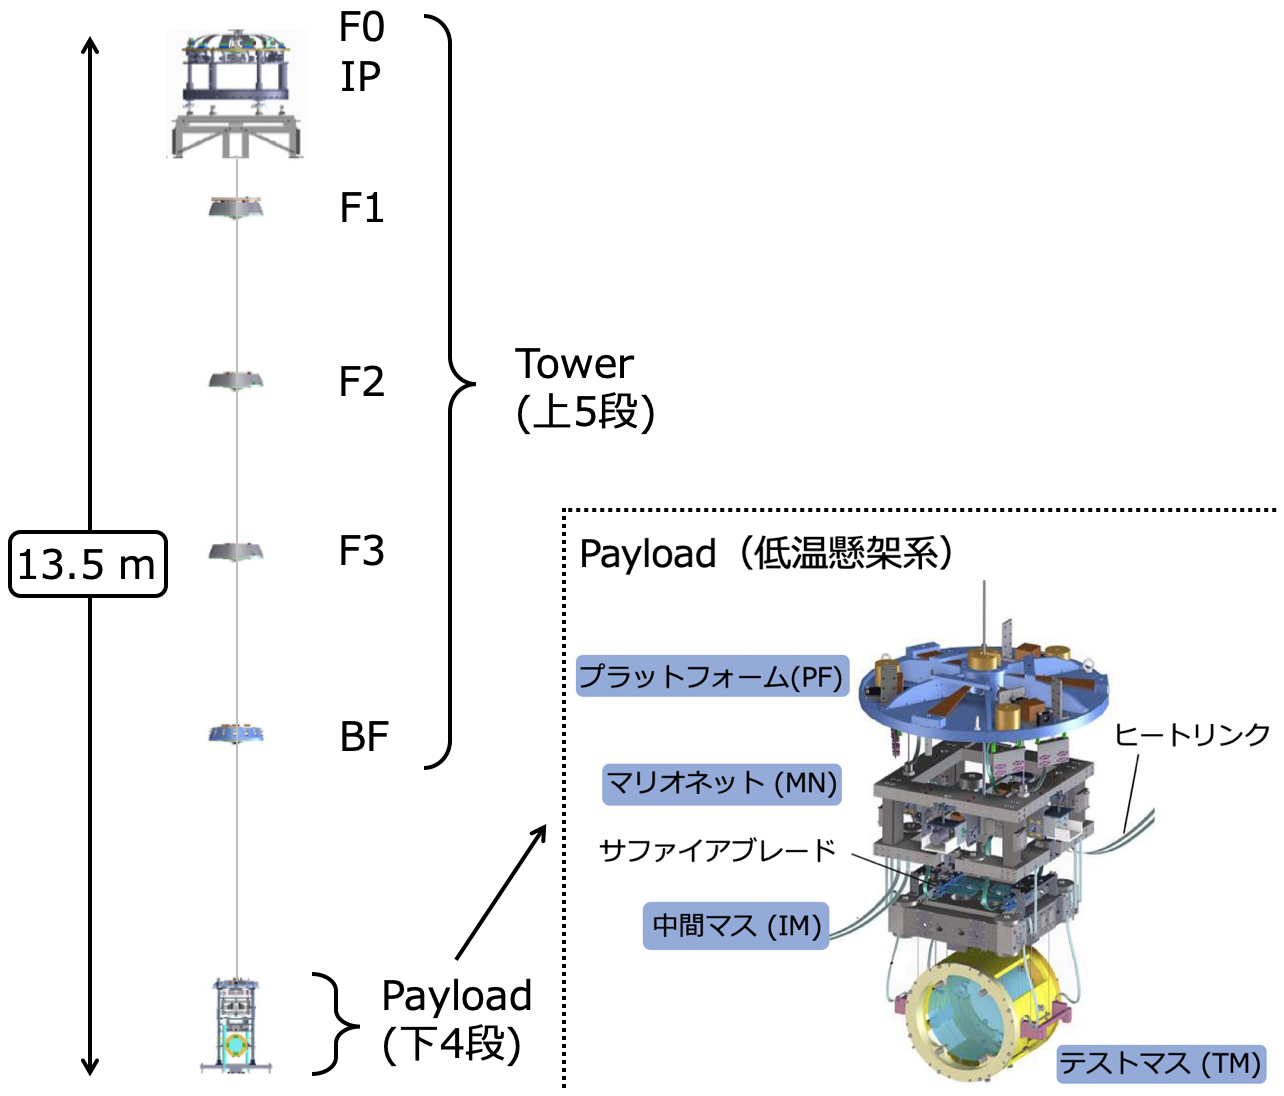
\includegraphics[width=150mm]{fig4_1.png}
\caption[Type-A Suspensionの全体図および低温懸架系部分]{Type-A Suspensionの全体図(左)および低温懸架系 (Cryogenic Payload) 部分(右下)}
\label{fig4.1}
\end{center}
\end{figure}

\section{Type-A Tower}
\subsection{機構}
Type-A Towerは主に1 Hz以下の低周波防振のための部分である. その構成について, IP pre-isolationステージは, 3本のIP (Inverted Pendulum) で支えられている. また, GASフィルタチェーンはトップステージに取り付けられたトップフィルタ(F0)から始まり, フィルタ1, 2, 3(それぞれF1, F2, F3)と名付けられた後続のステージが続き, BF (Botom Filter: ボトムフィルタ) と呼ばれる5段目で終了する. IPおよびGASの仕組みについては補遺\ref{補遺A}に記載した. 
\subsubsection{IP pre-isolation ステージ}
\vskip3mm
IP pre-isolationステージはプレアイソレータと呼ばれIP, ベースリング, トップGASフィルタ($\rm{F_0}$)で構成されている(図\ref{fig4.2}). このステージは0.1Hz以下の低周波からの防振, および防振懸架系全体の位置制御という役割を持つ. 
\begin{figure}[H]
\begin{center}
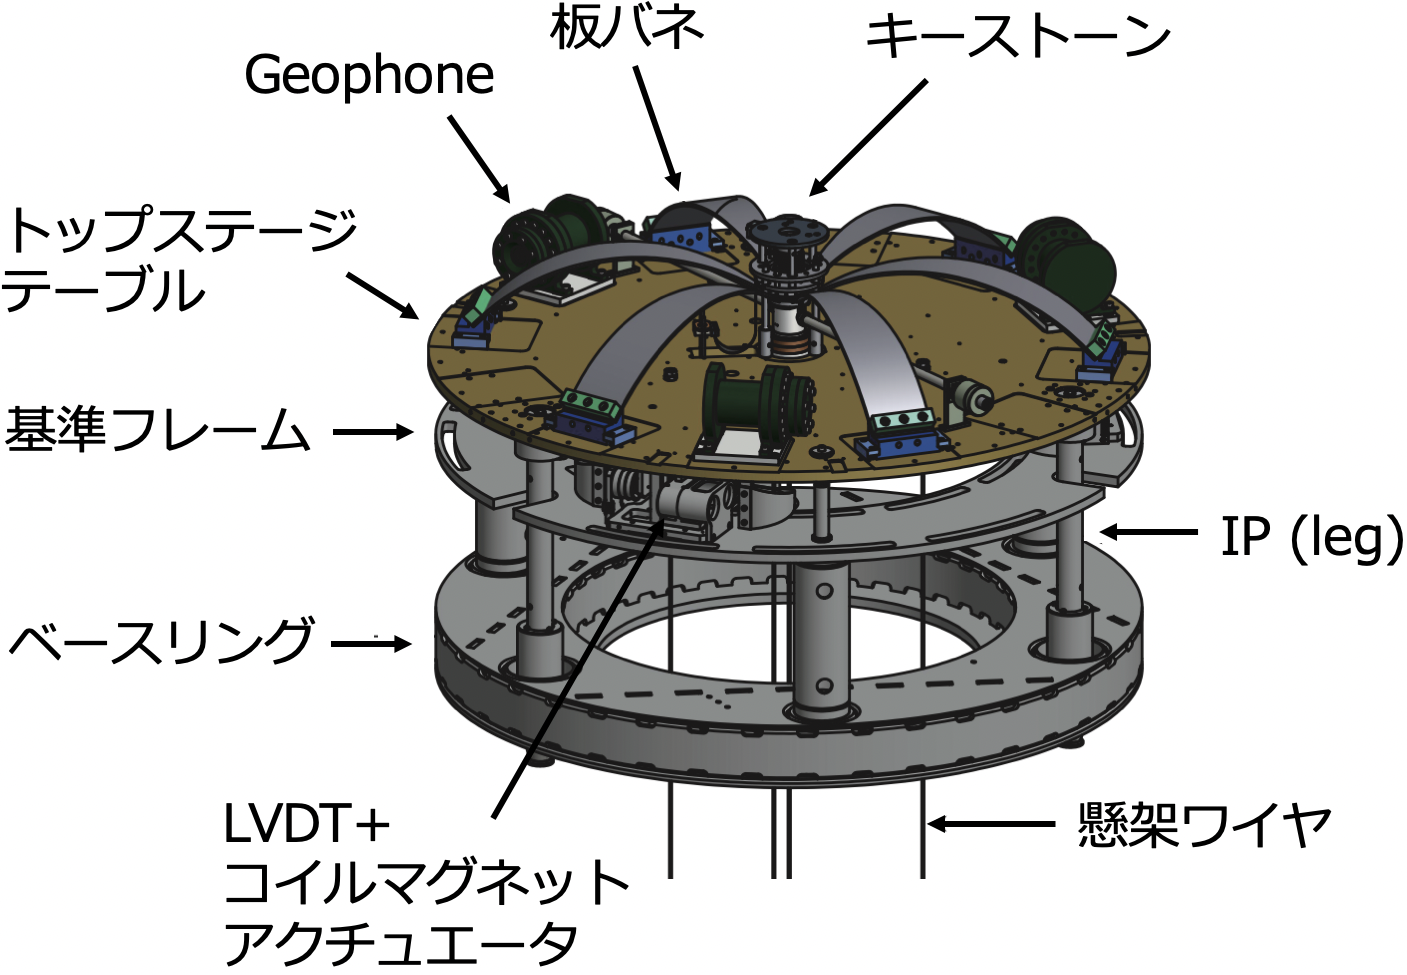
\includegraphics[width=130mm]{fig4_2.png}
\caption[IP pre-isolation ステージ]{IP pre-isolation ステージ(プレアイソレータ)}
\label{fig4.2}
\end{center}
\end{figure}
トップステージは3本のIPの脚で120$^{\circ}$ごとに支持されている. それらの間に位置する3本の支柱はベースリングと基準フレームを接いでおり, そこにLVDTとコイルマグネットアクチュエータのユニットが取り付けられている. また, 地面の揺れに依存しない慣性センサとして, 逆真空容器に収納されたgeophoneがトップステージに搭載されている. なお板バネの先端はトップフィルタの中央にあるキーストーンに接続されている. メインチェーンの懸架ワイヤの1本はこのキーストーンに繋がれており, 他の3本のmagnet damper用ワイヤはトップステージテーブルに直接接続されている. \\
\quad IPの脚は高さ520 mmであり, VirgoのSuper Attenuator\cite{Virgo}に使用されている高さ6mのものと比べてはるかに小さい. このIPは, 脚の中空円筒の両端にフレクシャ接合部を有している. フレクシャ接合部には, 優れた強度と靭性を持つマレージング鋼が使用され, 最上段の変位に伴う強固な弾性屈曲が可能になっている. 各IPはコーンベローズの上に立てられた上でスクリュージャッキにより支えられ, 高さを調節することで接地面を水平にしている. \\
\quad $\rm{F_0}$については, その構造と機能が他のGASフィルタと同様であるため, 次の小節で説明する. また, センサおよびアクチュエータについても後ほど記述する. 
\subsubsection{GASフィルタチェーン}
\label{sec4.1.1.2}
\vskip3mm
Type-A Suspensionには, 水平方向と垂直方向の両方の地面振動減衰を満たすために5段のGASフィルタチェーンがインストールされている. 最上段に実装されたGASステージはトップGASフィルタと呼ばれ, 続く3段はよりコンパクトな設計のGASフィルタ(標準GASフィルタ)になっている. なお, Tower部分の最終段はBF (Botom Filter) と呼ばれ, 基本的には標準GASフィルタと同じ機構だが, BFはTowerと低温懸架系の間のインターフェイスとして重要な機能を持つため, 区別されている. 
\begin{figure}[H]
\begin{center}
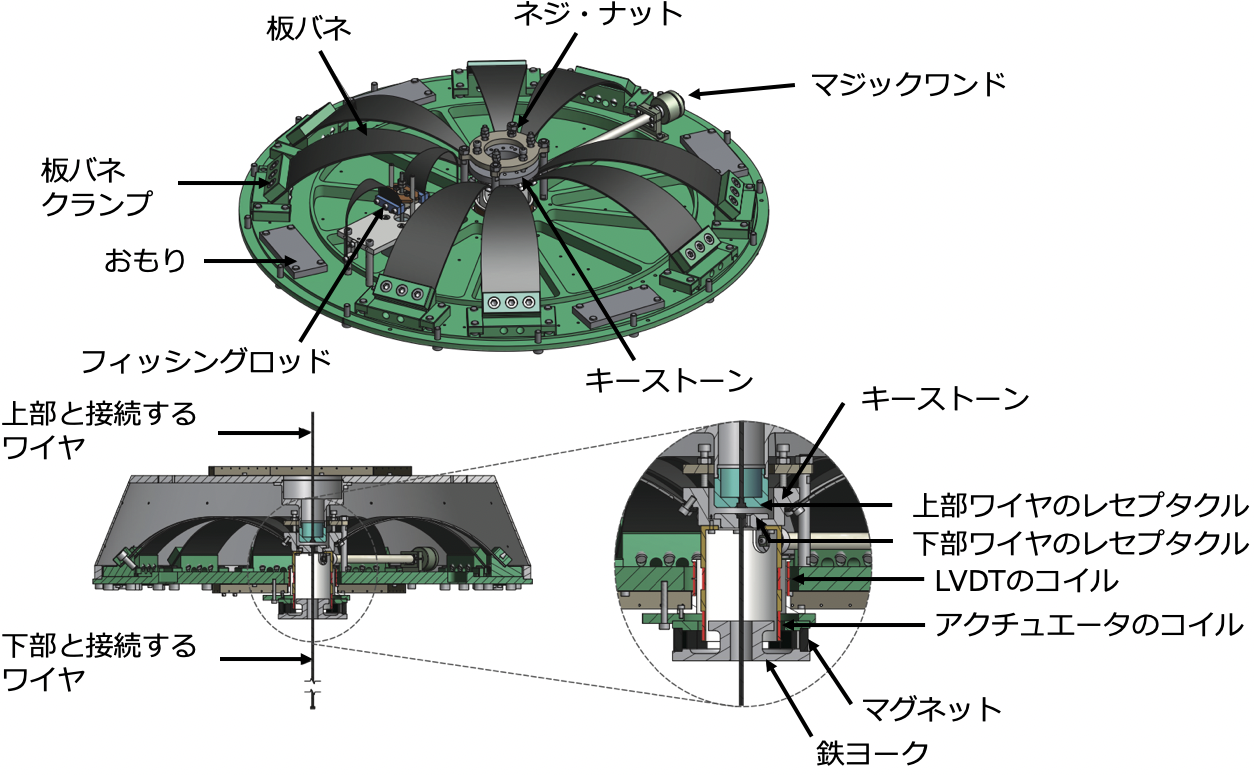
\includegraphics[width=160mm]{fig4_3.png}
\caption[GASフィルタ]{GASフィルタ}
\label{fig4.3}
\end{center}
\end{figure}
標準GASフィルタ($\rm{F_1},\rm{F_2},\rm{F_3}$)の基本構造は, 図\ref{fig4.3}に示すように円盤状のベースプレート上に実装されている(動作原理については補遺\ref{補遺A}に記した). 二等辺三角形の板バネが放射状にベースプレートに取り付けられており, 曲げられた板バネの先端は下段用の懸架ワイヤーが引っ掛けられるキーストーンに固定されている. これにより生まれる軸対称の制約から, キーストーンは垂直方向にのみ振動することができる. なお, その上下振動はLVDT変位センサでモニターしてコイルマグネットアクチュエータで制御している. また, 上段からのワイヤは三角錐型キャップの中心で引っ掛けられ, その半径方向の端でネジによってベースプレートに固定される. キーストーンとワイヤレセプタクルは懸架位置が質量中心に近くなるように配置されており, さらにキーストーンには振動中心を補正するためのマジックワンドが取り付けられている. \\
\quad また, 各板バネは曲がった状態で均一な応力分布になるように設計されている. さらに, その幅・厚み・枚数は, その最適荷重がステージからの吊り下げ重量と等しくなるように調整されている. 表\ref{table4.1}に示した通り, 重い荷重を支えるステージほど, 所定の共振周波数を得るために大きな反バネ効果が必要となるため, $\rm{F_0}$は板バネが厚く, また標準GASフィルタは上部のものほど板バネの枚数が多くなっている. 
\begin{table}[H]
 \centering
  \begin{tabular}{cccc}
   \hline\hline
    & 厚み [mm] & 最大幅 [mm] & 板バネの枚数 \\
   \hline 
   $\rm{F_0}$ & 5.0 & 125 & 6 \\
   $\rm{F_1}$ & 2.4 & 80  & 12 \\
   $\rm{F_2}$ & 2.4 & 80  & 10 \\
   $\rm{F_3}$ & 2.4 & 80  & 8 \\
   BF         & 2.4 & 80  & 5 \\
   \hline
  \end{tabular}
 \caption[GASフィルタの板バネのパラメータ(Type-A)]{GASフィルタの板バネのパラメータ(Type-A). $\rm{F_1,F_2,F_3}$が標準フィルタである}
 \label{table4.1}
\end{table}
\subsubsection{BF}
\vskip3mm
BFは, Type-Aサスペンションのタワー部にある最後のGASステージである. 基本的な機械設計は標準GASフィルタと同じだが, TowerとCryogenic Payloadのインタフェースとして特別な機能をいくつか持っている. \\
\quad BFの重要な役割の1つとして, 懸架系の下部において比較的大きな作動範囲の制御を行うことが挙げられる. このステージにはセンサ (BF LVDT) とアクチュエータが一体となったBF damperと呼ばれる装置が搭載されており, 地面に対するBFの動きを6自由度で測定し制御することができる. BFでは, アクチュエータから発生するノイズが鏡に伝わりにくいため, Payloadよりも大きな作動範囲を実現することができるのである. \\
\quad また, BF damperは単線懸架系のねじれ運動を減衰することができる. 懸架系のねじれは, 並進方向の地面振動と連動して発生する. そのためY方向には低周波の機械的共振によって十分な減衰が得られるので, 干渉計の感度に関わるノイズという観点ではねじり振動はあまり問題にならない. しかし, 懸架系がキックされてY方向の振動が励起されると減衰するのに長い時間を要し, 鏡の位置がずれて干渉計のデューティサイクルが低下する. BFの位置は基本Yモードのノード(上部のGASフィルタの懸垂点)から離れているため, BF damperを作動させることによって効果的なダンピングを適用できる. 
\subsection{センサ・アクチュエータ}
\ref{sec3.1}節で振り子による受動防振について述べた. しかし, 受動防振は共振周波数より高い周波数帯において地面振動の影響を抑えるものであり, 共振周波数付近およびそれ以下の帯域では能動防振が必要になる. これはセンサで読み取った振動を, アクチュエータで力を加えることにより減衰させるものである. 能動防振はセンサ・制御フィルタ・アクチュエータから成るが, この節ではType-A Tower部分で用いられるセンサおよびアクチュエータについて述べる(低温懸架装置で用いられるセンサ・アクチュエータは\ref{sec4.2.2}節, また制御フィルタについては第\ref{第6章}章参照). 
\subsubsection{LVDT}
\vskip3mm
LVDT (Linear Variable Differential Transducer) は誘導結合したコイル間の変調磁界を利用した相対変位センサであり\cite{36}(図\ref{fig4.4}), IPやGASフィルタの動きを読み取っている. その動作原理は次の通りである. \\
\quad 1次コイルに約10 kHzの正弦波変調信号を送ると, その周囲に振動磁界が発生する. そして, その磁界の変化を同軸上に置かれた2次コイルが感知し, 誘導電圧を発生させる. 2つの2次コイルは互いに逆巻きなので, 1次コイルを2次コイルの中心に置くと誘導電圧は打ち消される. ここで, 1次コイルが中心からずれると相互インダクタンスが変化し, 誘導電圧の差動がその後の読み出しで正味の電圧として現れる. この差動電圧は増幅されてミキサーに送られ, ミキサーはこの振動電圧を復調して1次コイルの変位(低周波信号)を得る. \\
\quad LVDTの特徴は変位に対する線形応答が, 軸方向の大きなダイナミックレンジで得られることである. KAGRAではそのダイナミックレンジはcm, 分解能はsub$\mu$mであるが, その具体的な値は用途によって決められる. KAGRA懸架系のシステムには, IPやGASフィルタに使用される標準的なLVDTとBFに使用される専用のLVDTの2種類があり, 後者についてはLVDTの2次コイルをアクチュエータコイルと共用する設計である. 
\begin{figure}[H]
\begin{center}
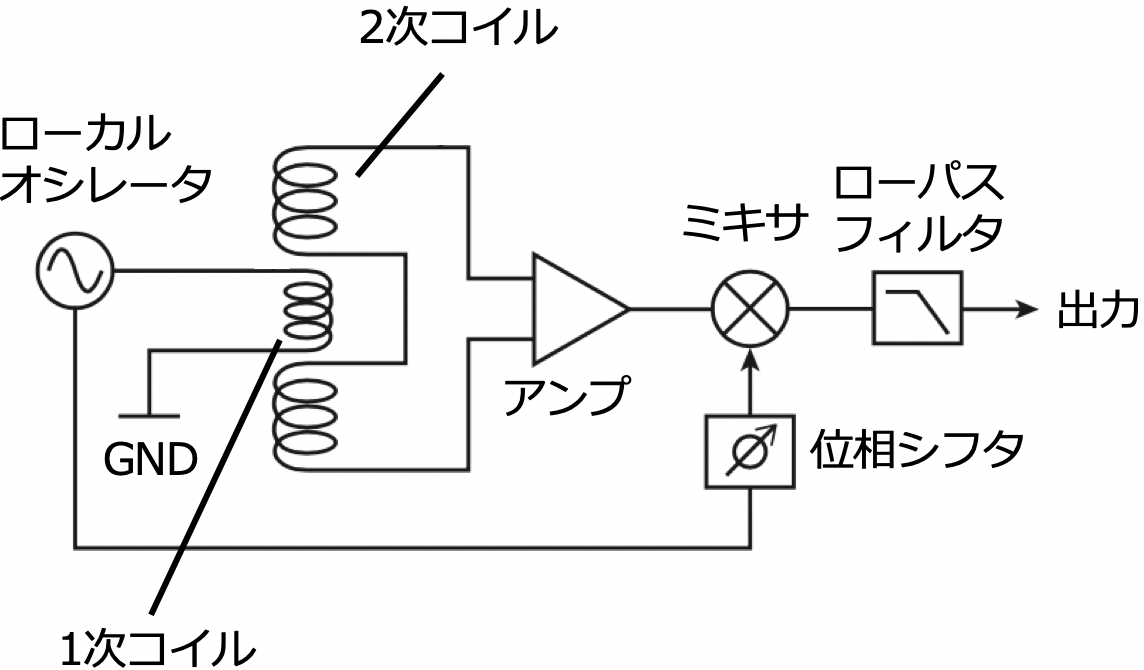
\includegraphics[width=130mm]{fig4_4.png}
\caption[LVDTの概要図]{LVDTの概要図}
\label{fig4.4}
\end{center}
\end{figure}
\subsubsection{Geophone}
\vskip3mm
Geophoneは慣性系に対する速度を測定する装置であり, LVDTと同様IPの動きをモニターする. 2種類のセンサを用いているのは, 感度が良い帯域が両者で異なるからである. 具体的には, GeophonはLVDTに比べ高い周波数で感度が良い. そのため, クロスオーバー周波数(両者のゲインの大小が入れ替わる周波数)が約0.1 HzとなるようにLVDTの信号にローパスフィルタを, Geophoneの信号にハイパスフィルタをかけてIPの制御を行っている. 図\ref{fig4.5}はその制御の様子を示したものである. LVDTのみによる制御(赤)では共振が抑えられているものの, 0.3 Hz以上でノイズが見られる. Geophoneを合わせることにより, そのノイズの影響が抑えられている(水色). 
\begin{figure}[H]
\begin{center}
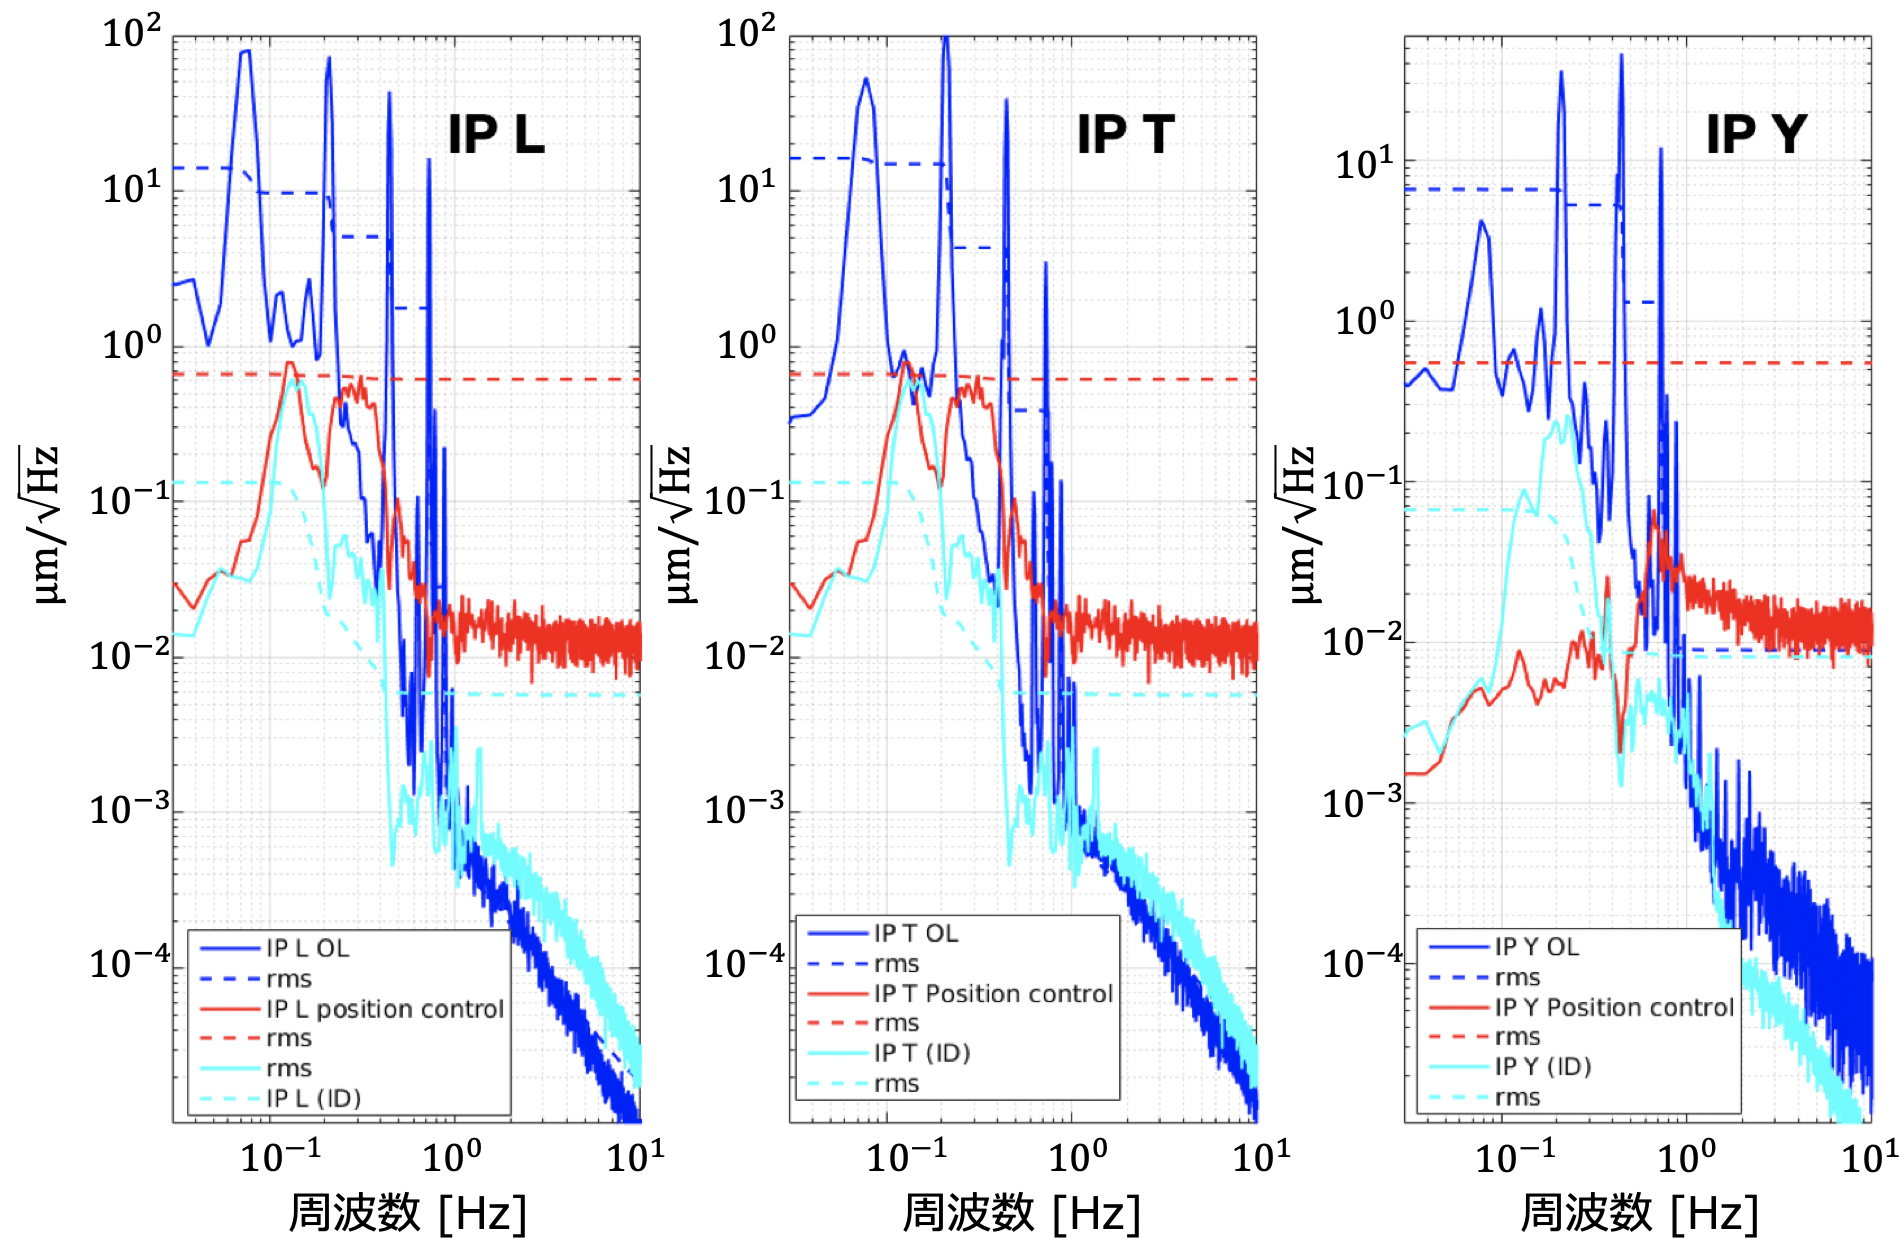
\includegraphics[width=160mm]{fig4_5.png} 
\caption[LVDTとGeophoneによるIPの制御]{LVDTとGeophoneによるIPの制御\cite{37}. 赤線はLVDTのみによる制御を示しており, 共振は抑えられているものの, 0.3 Hz以上でノイズが見られる. これにGeophoneを合わせた制御が水色であり, ノイズの影響が抑えられているのが分かる.}
\label{fig4.5}
\end{center}
\end{figure}
KAGRAではSercel社製のL-4Cを用いている. これはプルーフマスの筐体に対する速度に比例して電圧を出力するが, その動作原理は次の通りである. \\
\quad 約1 kgのプルーフマスはバネおよびdamperで吊り下げられており, コイルが巻き付けられている(共振周波数は1 Hz). そしてこのコイルが筐体に取り付けられた永久磁石による誘導電圧を発生させる. geophoneは特定の光や電波等の補助を必要としない受動計測装置であり, 内部発振器の制御を必要としないため設置やメンテナンスが容易である. \\
\quad generator定数$G_{\rm e}$, 減衰係数$\eta$, 角周波数$\omega$および角共振周波数$\omega_0$を用いるとgeophoneの周波数応答は
\begin{equation}
H_{\rm geo}(\omega)=\frac{G_{e}\omega^2}{\omega_0^2+2i\eta\omega_0\omega-\omega^2}.
\end{equation}
これよりgeophoneは共振周波数1 Hz以上では平坦な応答を示すが, それ以下の周波数では$f^2$に比例した周波数依存性を示すことが分かる(図\ref{fig4.6}). また, 各パラメータの典型的な値については表\ref{table4.2}の通りである. なお, これらのパラメータは, 複数種類の地震計による同時測定によって校正される. 特に, KAGRAでは地下施設の環境地震モニターとしてNanometrics社のTrillium Compactを2台, Trillium 120QAを1台使用している. これらは広帯域(0.01$\sim$10 Hz)でフラットな応答特性を持つため, 校正が簡単である. \\
\quad geophoneからの出力電圧は信号対雑音比を良くするために前置増幅器回路(プリアンプ)で増幅され, 制御システムに送られる. このとき, 雑音電圧が少ないオペアンプCS3002を用いた第1増幅段階で信号を374.5倍に拡大し, 第2増幅段階で2.5倍に増幅する. よって, 前置増幅器は合計約940 倍の増幅を行うことになる. なお, KAGRAではVirgo用にNikefで設計された前置増幅器回路を用いている. \\
\quad 一方, 前置増幅器はgeophoneの感度を制限するノイズを生む. 雑音電圧の測定結果より, 高周波(0.3 Hz以上)ではジョンソンノイズ(抵抗からの熱雑音), 低周波(0.3 Hz未満)では電流雑音(オペアンプからのノイズ)からの寄与があることが分かっている\cite{38}. 
\begin{figure}[H]
\begin{center}
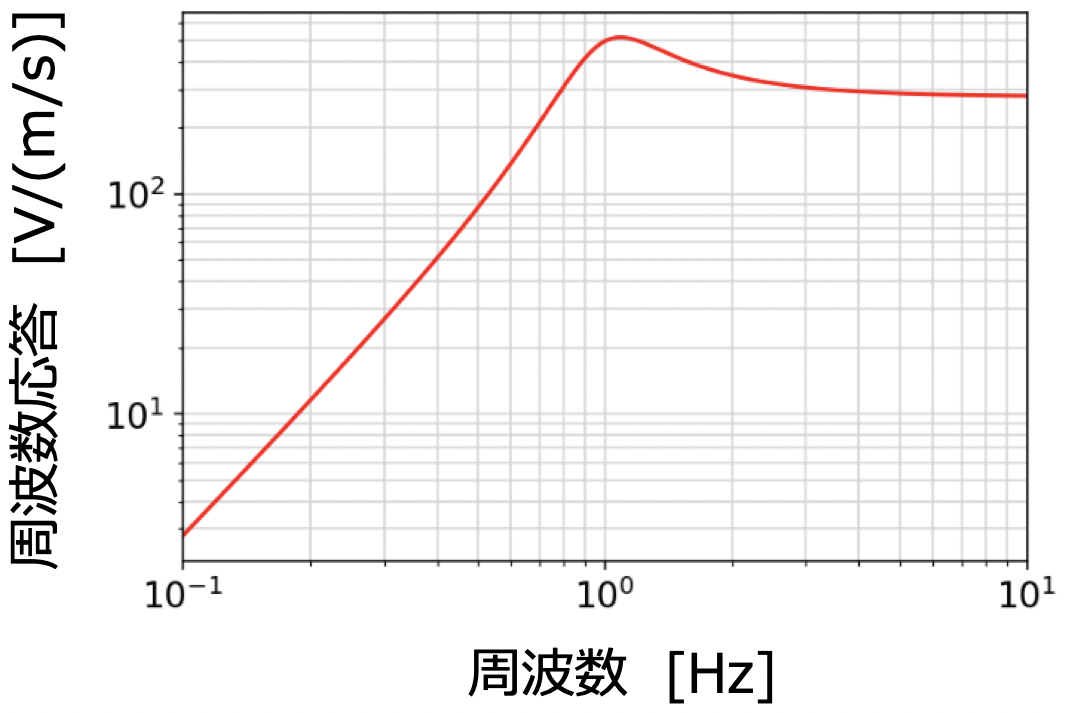
\includegraphics[width=120mm]{fig4_6.png} 
\caption[geophoneの周波数応答]{geophoneの周波数応答(フレーム速度から出力電圧への変換効率)}
\label{fig4.6}
\end{center}
\end{figure}
\begin{table}[H]
 \centering
  \begin{tabular}{cc}
   \hline\hline 
   generator constant & 276.8 V/(m/s) \\
   プルーフマスの重量 & 1 kg \\
   共振周波数         & 1 Hz \\
   減衰定数           & 0.28 \\
   コイルの抵抗       & 5500 $\Omega$ \\
   \hline
  \end{tabular}
 \caption[geophone (L-4C)の各パラメータ]{geophone (L-4C)の各パラメータ(典型的な値)}
 \label{table4.2}
\end{table}
また, geophoneと前置増幅器は大気中で動作させる必要があるが, 懸架系全体は真空中にある. そこで, geophoneの真空適合性を確保するため, ステンレス製の真空ポッドにgeophoneを封入して内部を大気圧に保った. なお, 真空ポッドからの空気漏れが数ヶ月のスケールで無視できることは, \cite{38}で示されている. また, 真空ポッド内のジオフォンの相対位置は, 読出信号に不要なインパルスを発生させる内壁のガタつきを防ぐため, ゴムリングで固定されている. このゴムリングの減衰効果は無視できるほど小さく, geophoneと真空ポッドの筐体は一体であると見なすことができる. 
\subsubsection{Folded Pendulum 加速度計}
\vskip3mm
LVDTとGeophoneを組み合わせてIPの制御を行うと述べたが, 図\ref{fig4.5}を見ると0.1 Hzあたりでの振動減衰は, IPのセンサへの要求値(0.1 Hzにおいて$10^{-7.8}$ m/$\sqrt{{\rm Hz}}$)に対して不十分である. これはGeophoneが低周波における感度が悪いため, クロスオーバー周波数を0.19 Hzまでしか下げられなかったことによる. \\\quad そこで, ノイズが要求に対して十分小さいことが先行研究\cite{FP}によって示されたFP (Folded Pendulum) 加速度計をインストールした. FP加速度計ではプルーフマスの一端を正立振り子で吊るし,もう一端を倒立振り子で支えている. 図\ref{fig4.7}はFP加速度計の概念図であり, このモデルでは質量$M_1$, 長さ$L_1$の正立振り子と質量$M_2$, 長さ$L_2$の倒立振り子が質量のない剛体梁で接続されている. この系の共振周波数は
\begin{equation}
\omega_0=\sqrt{\left(\frac{M_1}{L_1}-\frac{M_2}{L_2}\right)\frac{g}{M_1+M_2}+\gamma}.
\end{equation}
\begin{figure}[H]
\begin{center}
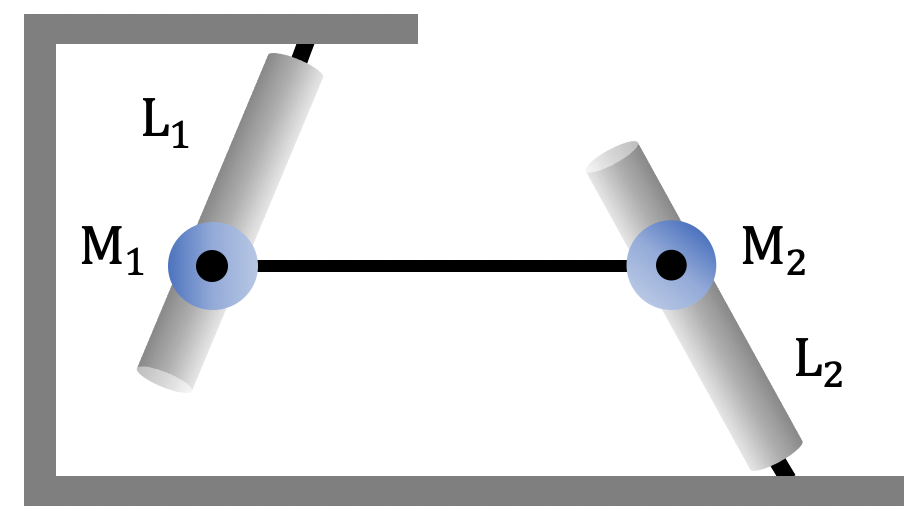
\includegraphics[width=120mm]{fig4_7.png} 
\caption[FP加速度計]{FP加速度計の概念図}
\label{fig4.7}
\end{center}
\end{figure}
\noindent
で与えられる($\gamma$はフレックスジョイントの剛性による影響を表す)\cite{39}. この共振周波数は, 2本のアームに対する重心位置を調節することで任意に下げることができる. \\
\quad KAGRAで用いるFP加速度計は幅140 mm, 高さ134 mm, 奥行き40 mmの大きさであり, IPの上にインストールすることができる. また, 真空中でも問題なく動作することも示されている\cite{FP}. 
\subsubsection{コイルマグネットアクチュエータ}
\label{sec4.1.2.4}
\vskip3mm
KAGRAのような重力波検出器では懸架された物体に力を加えるため, 真空で使える非接触のアクチュエータが必要になる. そこで永久双極子磁石とソレノイドコイルからなるコイルマグネットアクチュエータを用いる. これは永久磁石の静磁場とコイルに流れる電流の相互作用で発生する電磁気の力を利用したものであり, 十分な線形領域と作動力のダイナミックレンジを持つように設計されている. また, KAGRAの懸架系におけるコイルマグネットアクチュエータにはボイスコイル型と同軸可動磁石型の2種類があり\cite{41}, IPとGASには前者が, BFと低温懸架系には後者が用いられている. \\
\quad ボイスコイル型のアクチュエータは, 静磁場中を移動することでコイル内の電流がローレンツ力を受けるという作動原理である. 基準フレームに固定されている永久磁石(高透磁率の鉄製ヨークで成形されたもの)による一様な磁界の中にコイルのリード線が置かれ, ローレンツ力がコイル自身の作動力となる. \\
\quad 一方, 同軸可動磁石型のアクチュエータは永久磁石とソレノイドコイルが同軸に配置されており, 基準フレームに取り付けられたコイルの誘導磁界によって磁石に電磁力が加わる. 作動力の磁石の位置に対する依存性を軽減するために, 磁石はコイルの誘導磁界が十分均一である領域に配置されている. \\
\quad これらのアクチュエータでは常に最大作動力と雑音とのトレードオフがある. 大きな作動力を持つアクチュエータは, わずかな電気的変動でも雑音を生む. 特に防振懸架系の場合, 鏡に近いアクチュエータほど干渉計の感度に大きな影響を与える. そこで, KAGRAでは作動力とノイズの要件に応じて, 電流源と出力抵抗のオペアンプが異なる3種類のコイルドライバを使用している. Towerで用いられているものは表\ref{table4.3}に示した通りである. 
\begin{table}[H]
 \centering
  \begin{tabular}{ccccc}
   \hline\hline
   場所        & コイルドライバ & オペアンプ & 出力抵抗  & 最大電流 \\
   \hline
   IP・GAS・BF & ハイパワー     & OPA548     & 80 $\Omega$ & 0.12 A \\
   \hline
  \end{tabular}
 \caption[コイルドライバ(Tower)]{Towerで用いられているコイルドライバ. コイルのインピーダンスは出力抵抗には含まれていない. }
 \label{table4.3}
\end{table}

\section{低温懸架装置 (Cryogenic Payload)}
\subsection{機構}
BF以下は低温懸架系 (Cryogenic Payload) と呼ばれ, プラットフォーム(PF)から始まる. PFからはテストマス(TM)チェーンとリコイルマス(RM)チェーンの 2 つの3段振り子が並列に吊り下げられている. TMチェーンには上から順にマリオネット(MN), 中間マス(IM), テストマス(TM)という3つのステージがあり, RMチェーンはTMチェーンの対応するマスを取り囲むようなステージで, 地面の擾乱から隔離された作動力を加えることができる. 
\subsubsection{PF}
\vskip3mm
PFは低温懸架系の最上段にある円盤状のステージで, 長さ3.3 mのマルエージングワイヤでTower部分 (BF) と繋がっている(図\ref{fig4.8}左). PFには約4 Hzの共振周波数を持つベリリウム銅製の板バネが3枚取り付けられており, V方向の防振を行う. なお, TMチェーンはこの3枚の板バネが交わる点から吊るされている. また, PFからはRMチェーンがTMチェーンに並列に懸架されており, その回転を行うためのムービングマスがインストールされている(図\ref{fig4.8}右). 
\begin{figure}[H]
\begin{center}
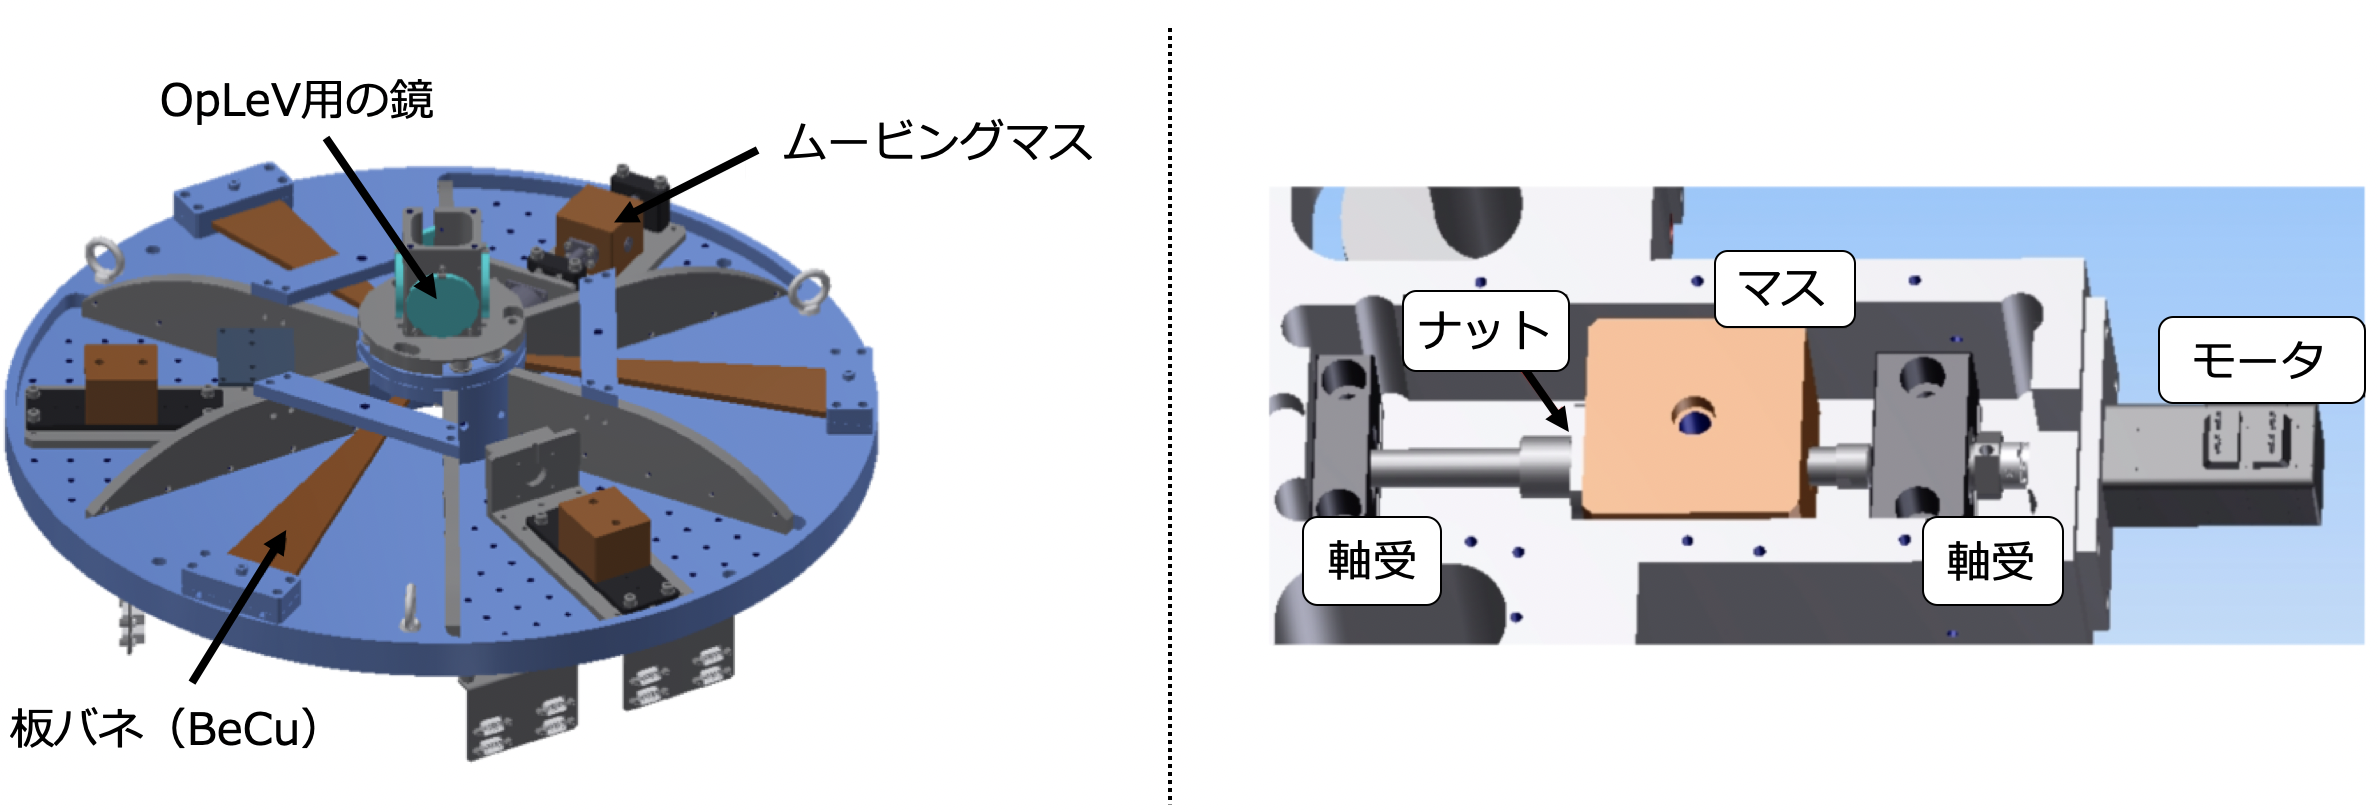
\includegraphics[width=150mm]{fig4_8.png} 
\caption[プラットフォーム (PF)とボールネジ型ムービングマス]{プラットフォーム (PF)とボールネジ型ムービングマス(ボールネジを用いてマスを動かす機構を持つ. ボールネジのナットがマスについているため, ネジの軸がモータによって回転するとマスがナットと共に動く. )\cite{42}}
\label{fig4.8}
\end{center}
\end{figure}
\subsubsection{MN}
\vskip3mm
マリオネット(MN)はTMチェーン初段の十字型ステージ(図\ref{fig4.9}左)であり, 回転自由度の剛性を低くするために質量中心に近い箇所を1本のマレージングワイヤで支持している. 干渉計の腕に沿った方向のMNの腕にはロープウェイ型ムービングマス(図\ref{fig4.9}右)が取り付けられており, MNの重心を変えることでTMのP方向の傾きを調節できる. なお, ボールネジ型のものを使用しないのは極低温かにおいて熱収縮によるスタックなど, ボールネジに起因する不具合が生じたからである\cite{42}. また, MNの下部にはOpLeV用の鏡があり, 外部からレーザーを当てることで, 地面に対するMNの角度をモニターすることができる(\ref{sec4.2.2.1}節および補遺\ref{補遺B}参照)\\
\quad 一方, マリオネットリコイルマス(MNR)はMNを囲むように取り付けられている(相対距離の初期値:20 mm). これは先述の通り3本のワイヤで懸架されているため, 1本のワイヤで吊られたMNに比べてY方向に揺れにくい. そこでMNRに設置されたフォトセンサによってMNとの相対位置を測定し, その信号をコイルマグネットアクチュエータ(MNに磁石・MNRにコイルがつけられている)にフィードバックすることによってダンピング制御を行っている(\ref{sec4.2.2.2}節および第\ref{第6章}章参照). 
\begin{figure}[H]
\begin{center}
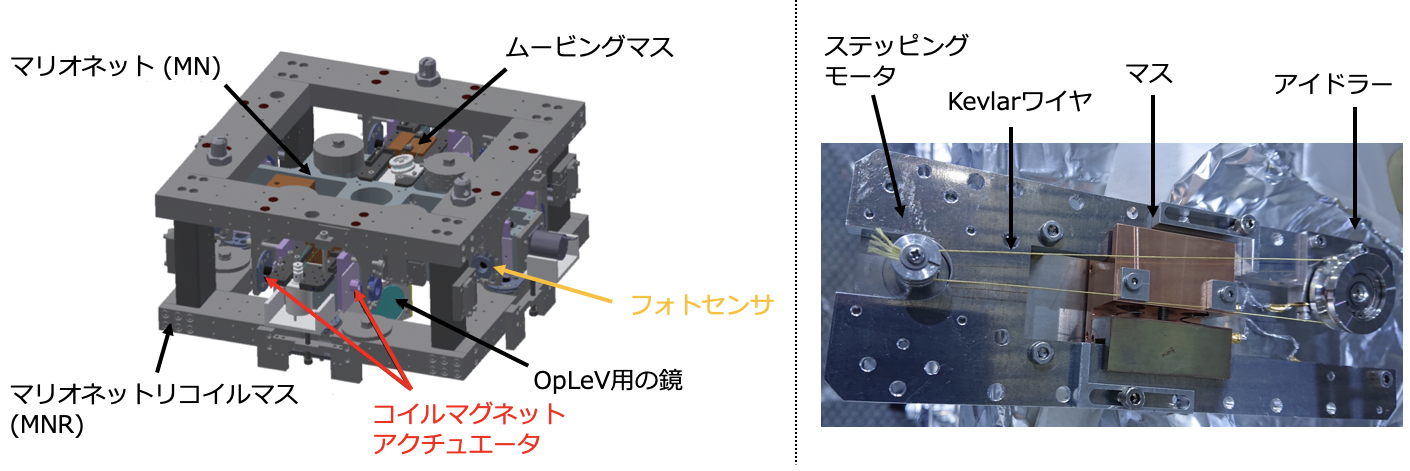
\includegraphics[width=180mm]{fig4_9.png}
\caption[マリオネット (MN)とマリオネットリコイルマス(MNR), およびロープウェイ型ムービングマス]{マリオネット (MN)とマリオネットリコイルマス(MNR), およびロープウェイ型ムービングマス(マス・Kevlarワイヤ・ステッピングモータ・アイドラーで構成されており, ワイヤとモータでマスを引っ張ることでMNの重心を変えている)\cite{42}}
\label{fig4.9}
\end{center}
\end{figure}
\subsubsection{IM}
\vskip3mm
中間マス(IM)はMNからベリリウム銅製のワイヤ4本で吊られている(図\ref{fig4.10}). IMにはサファイアブレード(サファイアファイバーを懸架するサファイア製の板バネで, ファイバーの縦方向の共振周波数を下げるほか, 長さのばらつきを補正する役割を持つ. )が取り付けられており, ミラーのV方向の防振を行っている. \\
\quad 中間リコイルマス(IRM)はMNRと同様, IMを囲むように取り付けられている(相対距離の初期値:20 mm). フォトセンサやコイルマグネットアクチュエータについてもMNRと同様で, MN段で制御できない固有モードも制御している. 
\begin{figure}[H]
\begin{center}
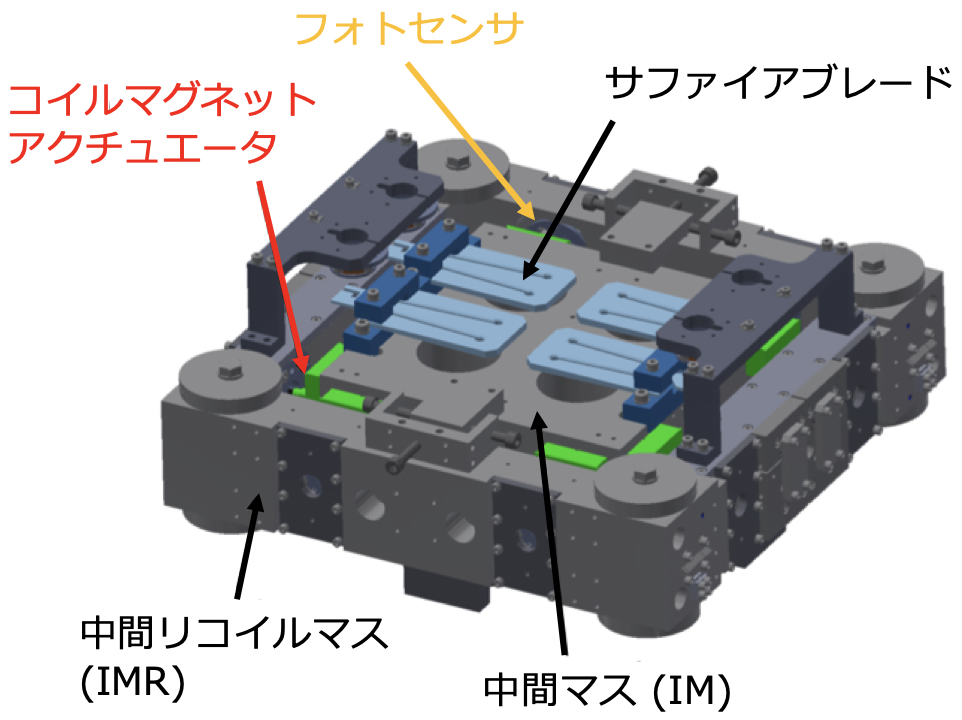
\includegraphics[width=90mm]{fig4_10.png} 
\caption[中間マス(IM)と中間リコイルマス(IRM)]{中間マス(IM)と中間リコイルマス(IRM)}
\label{fig4.10}
\end{center}
\end{figure}
\subsubsection{TM}
\vskip3mm
テストマス(TM)はサファイア鏡(直径220 mm・厚さ150 mm・質量23 kgの円筒形)であり, 低温懸架系の最下段に位置する(図\ref{fig4.11}). この鏡は低い熱雑音と高い熱伝導率を持ち, レーザー波長での高反射率, 低吸収率を実現させるため誘電体多層膜コーティングを施されている. しかしTMには常にレーザーが照射されることで熱を吸収し, 温度が上がってしまうので熱雑音が大きくなる. そこで直径1.6 mmのサファイアファイバー(TMの基材と同じ材料)4本で懸架し, 熱伝導率を向上させている. なお, ファイバーを引っ掛けるためにTMの側面2箇所にフラットカットを入れ, スリットが入ったイヤーと呼ばれるプリズムがHCB(Hydroxide Catalysis Bonding \cite{43})で取り付けられている. また, TMにもMNと同様OpLevが用いられているが, 地面に対する角度をモニターする Angle-sensing OpLev に加えて, 鏡の光軸方向の揺れを見るためのLength-sensing OpLev も設置されている. \\
\quad リコイルマス(RM)についてはMNやIMと同じく, TMを覆うように吊られており, TM・RM間のコイルマグネットアクチュエータで3自由度(L, P, Y)を制御している. 
\begin{figure}[H]
\begin{center}
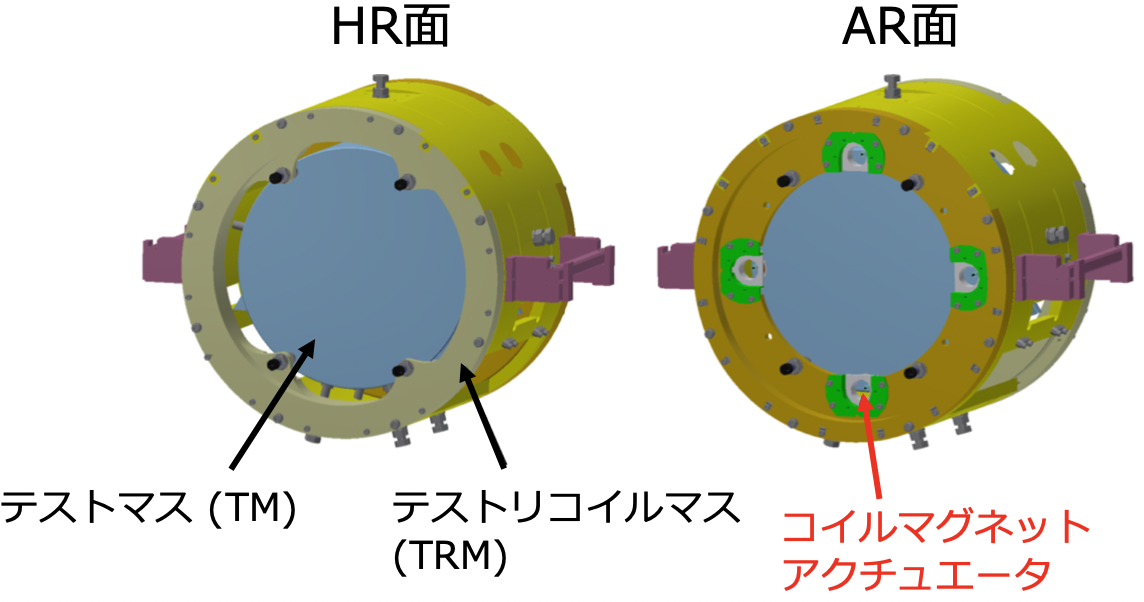
\includegraphics[width=130mm]{fig4_11.png} 
\caption[テストマス (TM)とそのリコイルマス (TMR)]{テストマス(TM)とそのリコイルマス(RM)}
\label{fig4.11}
\end{center}
\end{figure}
\subsection{センサ・アクチュエータ}
\label{sec4.2.2}
\vskip3mm
上述の通り低温懸架系の制御にはセンサとアクチュエータを用いる. MNとIMに関しては各自由度についてそれぞれフォトセンサでリコイルマスとの相対変位を測定できるようになっており, また, 地面に対する角度の測定はMNとTMに取り付けられた光てこを用いている. また, このアクチュエータで制御できる方向は図\ref{fig4.12}に示した通りで, MN・IMに関しては6自由度, 鏡に関してはL, P, Yの3自由度になっている. 以下ではそれぞれのセンサおよびアクチュエータについて簡単に記述する. 
\begin{figure}[H]
\begin{center}
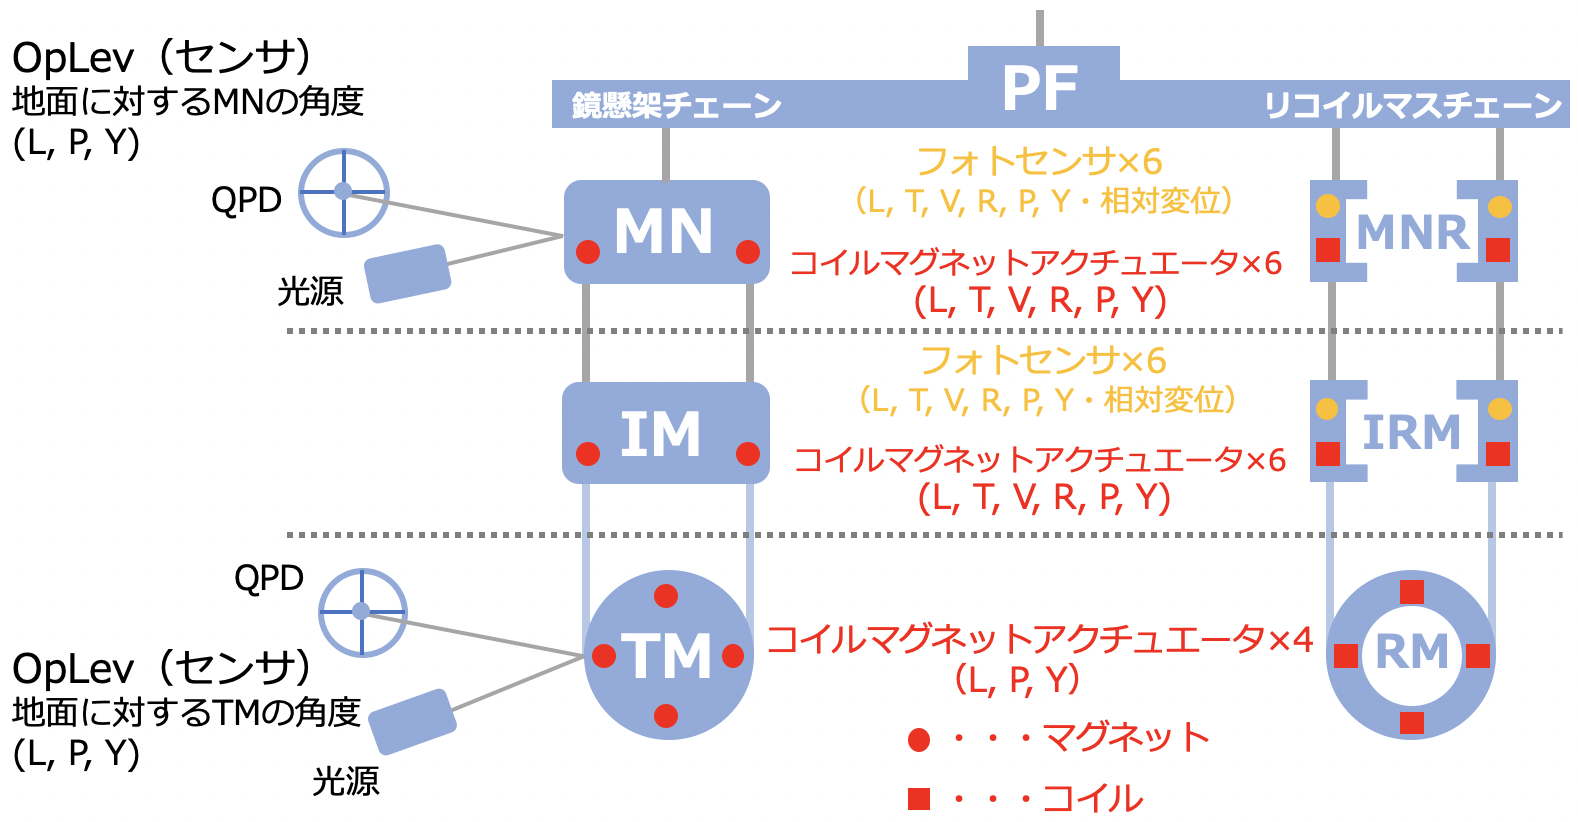
\includegraphics[width=160mm]{fig4_12.png} 
\caption[Payloadに関係のあるセンサ・アクチュエータ]{Payloadに関係のあるセンサ・アクチュエータ}
\label{fig4.12}
\end{center}
\end{figure}
\subsubsection{OpLev}
\label{sec4.2.2.1}
\vskip3mm
OpLevは鏡にレーザーを当てて, その反射光のビームスポットの位置を検知し, 鏡の地面に対する角度(水平)変位をモニターするものである. 低温懸架系ではMNにAngle sensing (角度方向の揺れを見る), TMにAngle sensingおよびLength sensing (水平方向の揺れを見る) OpLevを設置している. それらの原理については補遺\ref{補遺B}参照. また, 反射光の検知はQPD (Quadrant PhotoDiode) で行っている. 
\subsubsection{フォトセンサ}
\label{sec4.2.2.2}
\vskip3mm
センサには接触型のものと非接触型のものがある. 接触型センサは変位を高精度で読み取ることができるが, センサの振動がターゲットを揺らしてしまうので, KAGRAの懸架系に用いるのは不適切である. それに対し, 光や超音波を用いる非接触型センサは外乱を与える心配がない. \\
\quad そこで重力波検出器では非接触型のセンサを用いている. その中でも, 鏡を極低温まで冷却するKAGRAでは, 反射型のフォトセンサを用いている. これは反射型のフォトセンサがシャドーセンサ\footnote{マスの運動に伴ってフラッグがPDに入る光を遮る方向に動き, 光量の変化を変位として検出するセンサ. ダイナミックレンジが数 mmと小さいので冷却した際にフラッグがセンサに衝突して使用不可になる恐れがある. }などに比べてダイナミックレンジが広く, 冷却した際の熱収縮等でセンサが使えなくなる心配が少ないからである. \\
\quad 反射型フォトセンサはLEDおよび2つのPDから構成される. KAGRAではLED・PDを選定するための研究\cite{44}を行い,  Thorlabs社のInGaAs素子LED1200E\cite{45}をLED, InGaAsP製のFGA21\cite{46}をPDとして採用した. これはエネルギーバンドギャップの小さなInGaAsではエネルギーを媒介するキャリアとしてフォノンを使わない\footnote{フォノンは低温で励起しづらい. Siなどはエネルギーを運ぶキャリアがフォノンなので低温光学の分野では用いられない. }ので, 冷却した際も十分に動作できるからである. \\
\quad また, 反射型フォトセンサの動作原理は以下の通りである. LEDとPDは共にセンサに取り付けられており, LEDから出た光がターゲットで反射し, PDで検知される. このとき, 光軸方向のターゲット位置の変化に伴って反射光量も変化するので, そこからセンサ(リコイルマスチェーン側)とターゲット(鏡懸架チェーン側)の相対距離を割り出している(図\ref{fig4.13}右). 
\begin{figure}[H]
\begin{center}
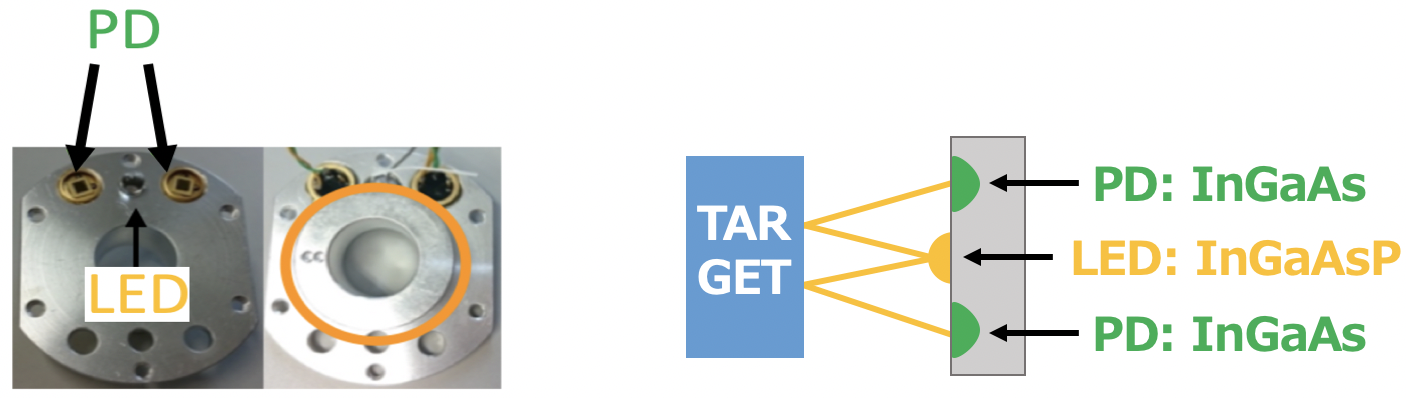
\includegraphics[width=170mm]{fig4_13.png} 
\caption[反射型フォトセンサとその動作原理]{実際にインストールされている反射型フォトセンサ(左)\cite{47}とその動作原理(右)}
\label{fig4.13}
\end{center}
\end{figure}
\subsubsection{コイルマグネットアクチュエータ}
\label{sec4.2.2.3}
\vskip3mm
低温懸架系で用いられるコイルマグネットアクチュエータは\ref{sec4.1.2.4}に示した通り, 同軸可動磁石型のものである. また, 低温懸架系の場合, 磁石がTMチェーンに, コイルがRMチェーンに取り付けられている. なお, 低温にしたときの特性の変化とバルクハウゼンノイズが小さいという理由でマグネットにはSmCo(サマリウムコバルト)を用いている. \\
\quad コイルドライバについては, 作動力とノイズのトレードオフを考慮し, MN・IMとTMで異なるものを使用している(表\ref{table4.4}). 
\begin{table}[H]
 \centering
  \begin{tabular}{ccccc}
   \hline\hline
   場所 & コイルドライバ & オペアンプ & 出力抵抗      & 最大電流 \\
   \hline
   MN   & ローパワー     & AD8671     & 1.4 k$\Omega$ & 9.5 mA \\
   IM   & ローパワー     & AD8671     & 1.4 k$\Omega$ & 9.5 mA \\
   TM   & ローパワー     & AD8671     & 7.8 k$\Omega$ & 1.3 mA \\
   \hline
  \end{tabular}
 \caption[コイルドライバ(低温懸架系)]{低温懸架系で用いられているコイルドライバ\cite{48}. コイルのインピーダンスは出力抵抗には含まれていない. }
 \label{table4.4}
\end{table}

\subsection{冷却システム}
低温懸架系は, 8 K innerシールドと80 K outerシールド\footnote{どちらもアルミニウム(Al1070)製で合わせて1400 kgある. また, 放射冷却をさらに向上させるため, innerシールドにはDLC(Diamond Like Coating)が施されている. }からなる二重構造のクライオスタットの中で, 4つの超低振動PTC(Pulse-Tube Cryocooler:パルス管冷凍機)を用いて冷却される(図\ref{fig4.14}). このPTCには2つの低温ステージ(それぞれ約40 Kと約4 Kに冷却する)があり, それぞれがVR(Vibration Reduction:振動減衰)ステージに熱的に接触している. また, PTC-1, 2, 3, 4の1段目はouterシールドに, PTC-2と4の2段目はinnerシールドに接続されている\cite{49}. 
\begin{figure}[H]
\begin{center}
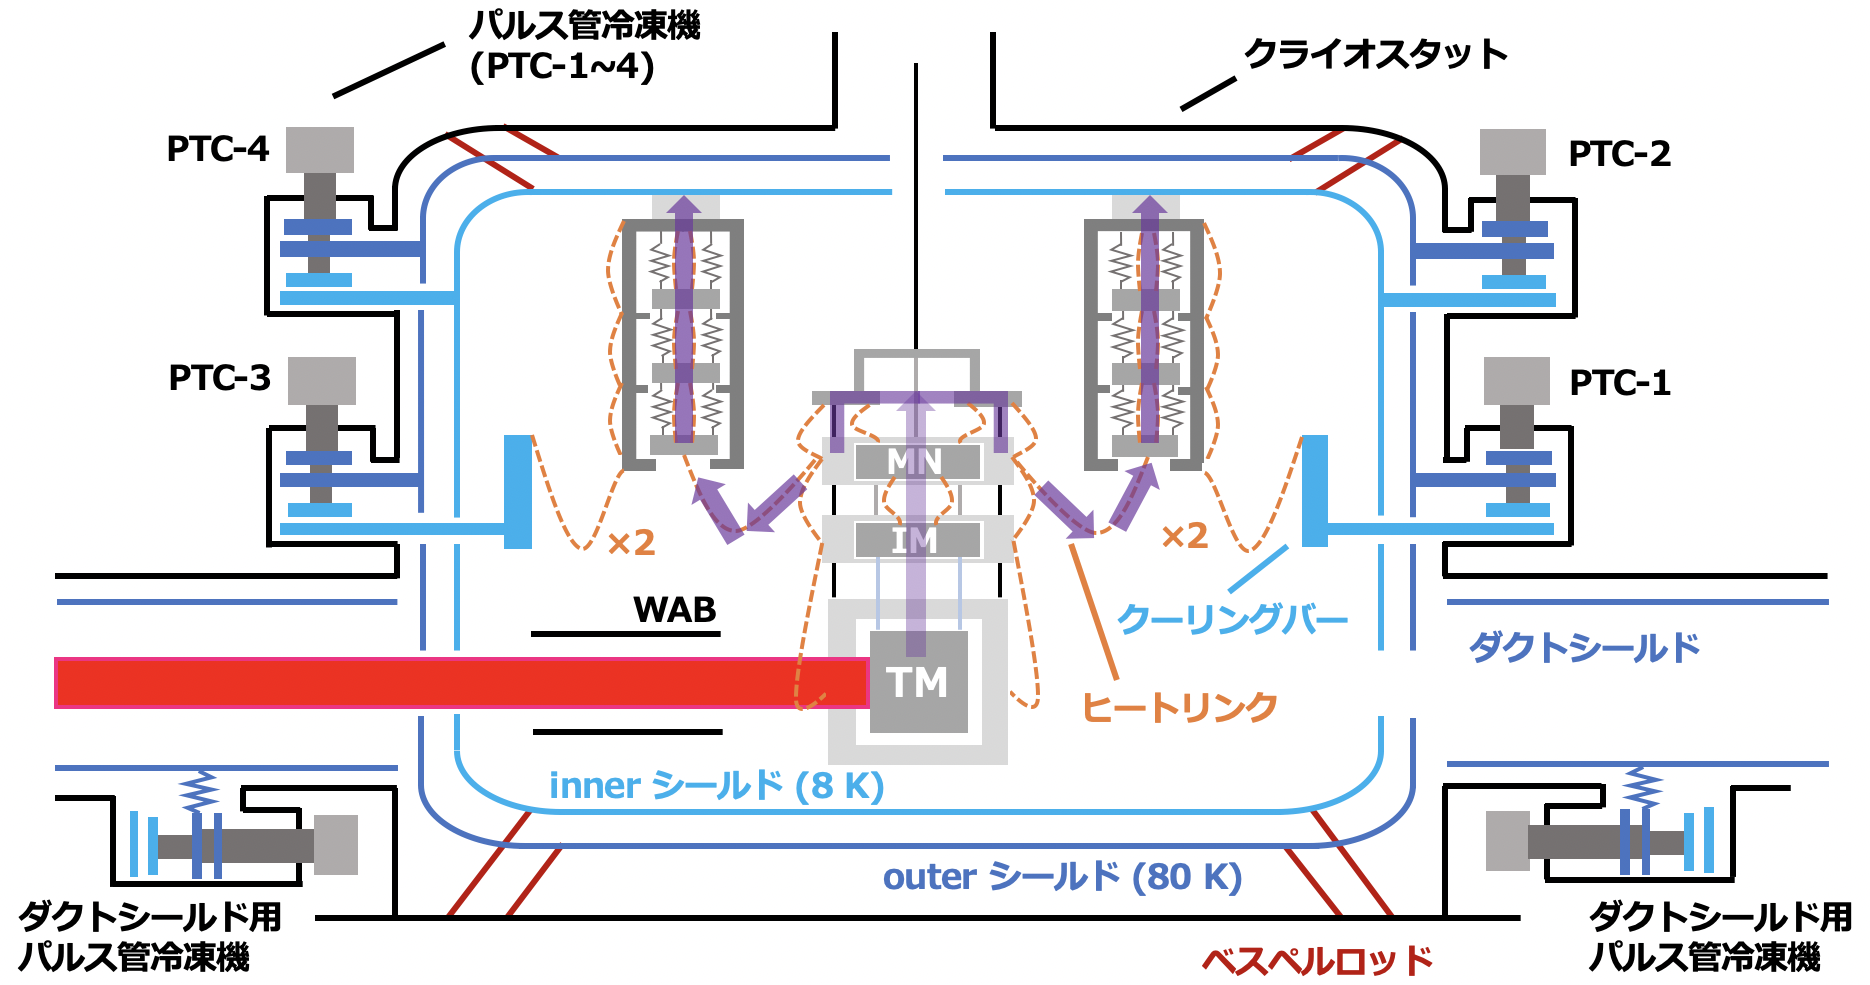
\includegraphics[width=170mm]{fig4_14.png} 
\caption[低温懸架系の冷却システム]{低温懸架系の冷却システム. 低温懸架系は二重放射シールドを持つクライオスタット内で冷却される. 1番外側の黒が逆真空容器, 内側の青は80Kと8Kの放射線シールドを示している. 80KシールドはPTC-1,2,3,4の1段目で冷却され, 8KシールドはPTC-2と4の2段目で冷却される. PTC-1と3の2段目はクーリングバーに接続され, 6N Al製のヒートリンクを通して低温懸架系を冷却する. また, クライオスタットの左右にあるダクトシールドは, 1段のPTCで120Kまで冷却される. }
\label{fig4.14}
\end{center}
\end{figure}
低温懸架装置の冷却における熱伝達経路は放射冷却と伝導冷却の2つに分けられる. まず放射冷却について, 先に示した二重の放射シールドは八角柱の構造で, 300 Kの外部放射から低温懸架装置を隔離して冷却する. このシールドからの熱放射により, 低温懸架装置は約100 Kまで効果的に冷却される. また, レーザーの光路を作るシールドの両脇の穴も熱放射源となる. この穴からの300 Kの放射を最小限にするため, 左右に5 mのダクトシールドが設置されており, それぞれのダクトシールドはダクトシールド用のPTCの1段目によって120 Kまで冷却される\cite{49}. \\
\quad 次に伝導冷却について, Payloadの各ステージはヒートリンクと呼ばれる6N (6 Nine, すなわち99.9999$\%$) のAlのケーブルで接続され, 伝導冷却が行われる\cite{50}. TMに吸収された熱は上段へ流れ, 最終的にヒートリンクとAl クーリングバーを通してクライオスタットへ抽出するという仕組みである. この機械的伝導経路は, 各ステージにさらなる振動を引き起こす可能性があるため, MNRに取り付けられたヒートリンクを中継する3段の防振系がクライオスタットに実装されている. この伝導冷却によって, TMの温度を20Kまで下げることができる. \\\\
\noindent
第\ref{第5章}章以降ではこのType-A Suspensionの内, 特に低温懸架系の特性評価および制御について記述する. 